\section{Introdução}\label{sec:intro}

\indent A agricultura brasileira desempenha um papel estratégico na economia nacional, sendo responsável por aproximadamente 23,2\% do Produto Interno Bruto (PIB) em 2024 \cite{cna2025}. No DF, em 2024, cerca de 21\% das exportações estaduais foram produtos agrícolas \cite{dataviva-graph-2025}; uma participação econômica significativa, possivelmente apontando que uma otimização do modelo de produção adotado poderia beneficiar não só os produtores, mas o restante da sociedade.


Um conceito recente na forma como se dá a produção agrícola é a agricultura de precisão, precisão obtida pela utilização de recursos tecnológicos e computacionais de ponta para a obtenção de métricas e análises e subsequente otimização dos recursos utilizados e resultados obtidos durante a produção \cite{tschiedel_ferreira_2002}.


O objetivo do trabalho apresentado por meio desse relatório é o projeto e execução de um protótipo de sistema computacional integrado com sensores capazes de prover análises simples para seu usuário utilizando técnicas de machine learning, tais como redes neurais. Em outras palavras, este trabalho propõe o desenvolvimento de uma estação meteorológica compacta para os fins de coleta e análise de dados, capaz de comunicar ao usuário final do sistema possíveis alertas e resultados. Além de já demonstrar resultados em outras áreas, redes neurais aplicadas a um ambiente rural aparentam ser um tópico em constante progresso \cite{machine_learning_in_agriculture}, permitindo uma oportunidade de estudo de vantagens e dificuldades apresentadas durante o desenvolvimento do sistema pretendido.


Para esse fim, utilizaremos um SoC(System on a Chip) Raspberry Pi 4 \cite{rpi4} e sensores específicos de temperatura, umidade, pH, entre outros, a serem detalhados posteriormente, capazes de coletar dados climáticos e ambientais voltados para a aplicação agrícola. Além disso, o sistema incorpora um modelo de inteligência artificial que processa os dados localmente e envia os resultados para um servidor, possibilitando a visualização em dashboards interativos.

\begin{figure}[!htpb]
    \centering
    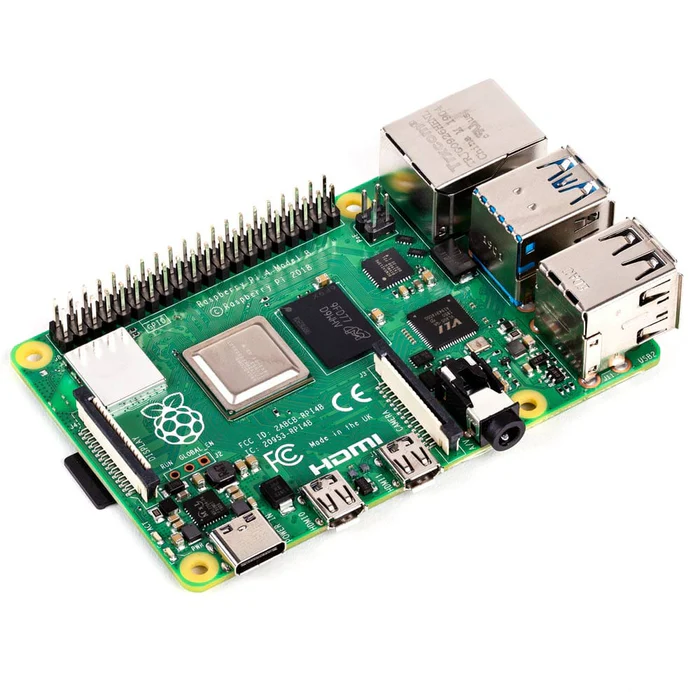
\includegraphics[width=.9\columnwidth]{figuras/rpi4.png}
    \caption{Raspberry Pi 4 Modelo B~\cite{rpi4}.}
    \label{fig:rpi4}
\end{figure}

\newpage

% Este documento \LaTeX~foi organizado em uma série de arquivos separados para cada Seção, localizados na pasta \texttt{editaveis}. 
% Confira ao longo dos arquivos como incluir
% figuras como a Fig. \ref{fig:rpi3}, além de tabelas, notas de rodapé e referências.
% Para acrescentar referências, altere o arquivo \texttt{editaveis/refs.bib}, que segue o formato BibTeX~\cite{ref:bibtex}. 

% Para manter o projeto organizado, acrescente suas figuras à pasta \texttt{figuras}. 
% % Confira no arquivo \texttt{editaveis/02\_introducao.tex} como incluir figuras como a Fig. \ref{fig:rpi3} e tabelas como a Tabela \ref{tab:pontuacao}.
% Para figuras e tabelas, não se preocupe com o posicionamento delas no texto. 
% O importante é que todas sejam referenciadas, assim como foi feito na segunda linha deste parágrafo.

% Todo o texto deve ser auto-contido; isto é, ele deve se explicar por si só. As figuras e tabelas somente \textit{auxiliam} no entendimento do texto. Sempre que o autor tiver que se explicar após a escrita, isto significa que o texto não está claro.

% O projeto completo deverá ser desenvolvido em ambiente Git público (GitHub, GitLab etc.), incluindo cronograma do projeto, código-fonte, código \LaTeX~deste relatório e resultados (planilhas, fotos etc).
% O repositório do projeto terá dois propósitos: servir de portfólio para os integrantes do grupo, e estender os conhecimentos de sala de aula para a comunidade em geral (créditos de extensão).


